
% here we go agane

\documentclass{article}

\usepackage[utf8]{inputenc}

\usepackage{amsmath, bm}
\usepackage{graphicx}
\usepackage{amssymb}
\usepackage{float}
\usepackage{caption}
\usepackage{subcaption}
\usepackage{hyperref}
\usepackage{tikz}
\usepackage{layout}
\usepackage{wrapfig}

\usepackage[margin=1in]{geometry}
\usepackage{listings}
\usepackage{xcolor}
\usepackage{color, colortbl}
\usepackage{textgreek}
\usepackage{mathrsfs}

\usepackage[moderate]{savetrees}

% 12 pt font
\renewcommand{\normalsize}{\fontsize{12pt}{\baselineskip}\selectfont}

\begin{document}

\title{4A7 Report \\ Climate Impact of Contrail Avoidance}
\author{5739G}
\date{December 2024}
\maketitle

\section{Introduction}
% evaluate the net climate impact of contrail avoidance
Understanding the role of aviation on climate impact is vital as it plays a significant contribution to global warming.
Simple models can provide insight into large scale effects on climate and will be used here to analyse the effectiveness of contrail avoidance. 

\section{Objectives}

\begin{itemize}
    \item Understand and quantify the climate impact of contrail avoidance using simple contrail and climate models.
    \item Investigate the impact of different aircraft fleets and fuels on the climate impact of contrail avoidance.
    \item Discuss limitations of simple models and compare to more complex models within the literature.
\end{itemize}

\subsection{Cases}

\begin{itemize}
    \item Baseline case, contrail avoidance with current aircraft fleet.
    \item If the aircraft fleet is assumed to instead be fueled by liquified natural gas (LNG), which is taken to be methane
    \item If the gas turbines powering the fleet have a higher thermal efficiency (by an amount of your choosing) 
\end{itemize}

\section{Simplified Model}

The model consists of multiple coupled differential equations that are solved numerically.

\subsection{Radiative forcing from emissions}

The kerosene fuel burned by aircraft contains a mixture of alkanes of varying carbon chain lengths.
The combustion of each of these alkanes can be weighted by concentration to obtain an overall
emissions index of 3.15 in units mass of $CO_2$ per mass of kerosene fuel burned.
To get the total mass of fuel burn its required to know the flight paths and fuel burn rates for all aircraft.
This simply wasn't possible for all aircraft and times and so a months commercial flights dataset from EUROCONTROL [?] was used with a smaller list of aircraft cruise fuel burn rates (kg/km) from wikipedia [?].
A correction factor was used to extrapolate the mass of fuel burned for unknown aircraft which was the ratio of total distance flown by all aircraft to aircraft of known fuel burn rate.
The CO2 emissions from flight was then estimated to be 0.31 Gt/Year.
Avoidance will come at a cost of an additional 1\% fuel consumption, compared to direct flight passing through the contrails.

The radiative forcing due to aircraft emissions of greenhouse gases can be estimated using the following simplified method.
In literature common units for carbon coming into or going out of the atmosphere is billions of tons of carbon per year ($\text{GtCyr}^{-1}$)
denoted $E(t)$, at the time $t$ in years. The carbon content of the atmosphere in units of billions of metric tons of carbon is denoted $C(t)$.
The current year is denoted $t=0$.
Measurements of E(t) and C(t) show that only roughly half of carbon emissions stay in the atmosphere, the rest is absorbed by the ocean and biosphere \cite{co2_modelling}.
This empirical observation is captured by the \emph{Constant Airborne Fraction Model}:

\begin{equation}
    \frac{dC}{dt} = k \left( E(t) - \frac{C(t)-C_\text{pre}}{\tau}\right)
\end{equation}

Where $k = 0.449$, $\tau = 276 $ years and $C_\text{pre} = 600$ GtC \cite{co2_modelling}.

Radiative forcing can be estimated using a relation by G. Myhre \cite{rf_greenhouse}.
This term adds a nonlinearity to the system of equations and is the reason for solving them numerically.

\begin{equation}
    \text{RF}_{\text{CO}_2} = 5.35 \ln \left( \frac{C}{C_0} \right) \label{eq:rfco2}
\end{equation}

Additional net radiative forcing due to NOx emissions is estimated by D.S. Lee et al. at $17.5mW/m^2$

\subsection{Contrails}

The radiative forcing due to contrails is also taken from the work of D.S. Lee et al. \cite{contrail_radiative_forcing}.
An effective radiative forcing is taken as 57.4 mWm$^{-2}$.


\subsection{Temperature response}

These radiative forcing values provide an instantaneous metric for climate impact of emissions, however
the temperature response is a cumulative effect of radiative forcing over time.
This can simply be modelled by two heat reservoirs, one for shallow ocean and one for the deep ocean.
The temperature of the atmosphere $T_1$ and the temperature of the ocean $T_2$ are then given by the following equations.

\begin{align}
    C_1 \frac{dT_1}{dt} &= A_E[\text{RF} - \lambda(T - T_0) - k_m(T_1 - T_2)] \\
    C_2 \frac{dT_2}{dt} &= A_E[k_m(T_1 - T_2)]
\end{align}

Where $\lambda$ is the climate sensitivity parameter, $T_0$ is the pre-industrial temperature, $k_m$ is the heat exchange coefficient between the atmosphere and the ocean, and $C_1$ and $C_2$ are the heat capacities of the atmosphere and ocean respectively.
The values of these are set in table \ref{tab:temp_model_params}.

\begin{table}[H]
    \centering
    \begin{tabular}{cccc}
        \hline
        Parameter & Value & Unit & Source\\
        \hline
        $T_0$ & 288 & $^\circ K$ & \\
        $\lambda$ & 1.0 & $W/m^2K$ & \\
        $k_m$ & 1.0 & $W/m^2K$ & \\
        $C_1$ & $7.4\times 10^{22}$ & J/K & $\rho c_p A_o \cdot 50$  \\
        $C_2$ & $5.3\times 10^{24}$ & J/K & $\rho c_p A_o \cdot (D_o - 50) \footnotemark $\\
        \hline
    \end{tabular}
    \caption{Temperature model parameters}
    \label{tab:temp_model_params}
\end{table}

\footnotetext{$A_o$ is area of earths oceans, $D_o$ is average ocean depth}

AGWP can quantify cumulative radiative forcing.
AGTP can quantify the cumulative impact of increased temperatures such as changes in ecosystems and sea levels.
\begin{align}
    \text{AGWP} &= \int_0^T \text{RF}(t) dt \\
    \text{AGTP} &= \int_0^T \Delta T(t) dt
\end{align}

\subsection{Adaption for LNG fuel}

Liquid natural gas fuel will be taken as methane which has an emissions index lower than kerosine
of 2.75 kg $CO_2$ per kg methane burned.
This means a smaller emissions penalty of additional fuel consumption by avoiding contrails.

The Schmidt-Appleman criterion predicts contrails form if the mixture of exhaust gases and ambient air
transiently reaches or surpasses saturation with respect to liquid water.
It can be shown that the gradient of the mixing line is proportional to the $H_2O$ emissions index (ratio of mass $H_2O$ released per kg fuel burned) and inversely proportional to $LCV$ (Equation \ref{eq:SAC_gradient}).
Methane has a slightly higher calorific value $LCV$ ($50MJ/kg$) than kerosine ($43MJ/kg$) however the water vapour emissions index of methane (2.25) is significantly higher than kerosine (1.29).
By aligning this increased gradient to the saturation curve shows that contrails can form at higher temperatures.
Hence, more contrails form and cause a larger net radiative forcing making their avoidance more important.

However, to estimate the increased radiative forcing, the previous value by D.S. Lee et al. was multiplied by the ratio
of mixing line gradients.

\begin{equation}
    G = \frac{P \cdot EI_{H_2O} \cdot c_p}{\epsilon \cdot LCV \cdot (1-\eta)} \label{eq:SAC_gradient}
\end{equation}

Where P is static pressure, $c_p$ is specific heat capacity, $\epsilon = M_{H_2O}/M_{air} = 0.622$, $LCV$ is lower calorific value, and $\eta$ is thermal efficiency.

\subsection{Adaption for higher thermal efficiency}

A higher thermal efficiency reduces amount of fuel required for a flight, reducing the emissions.
However, it also reduces the term $(1-\eta)$ which G is inversely proportional and so the SAC mixing curve gradient increases.
Again this means that more contrails form and so avoidance may be more worthwhile for aircraft of higher thermal efficiency.

An increase in thermal efficiency from 0.5 to 0.52 will be considered.
This may seem very small but actually represents a significant advancement from current technology.
To estimate the increased radiative forcing the same technique as before where the value by D.S. Lee et al. was multiplied by the ratio
of mixing line gradients.


\subsection{Assumptions and Limitations}

Many assumptions and simplifications were made to perform the above analysis.
The validity of these are discussed with reference to more advanced models.

Emissions
\begin{itemize}
    \item Kersoine fuel is free of impurities and has an CO2 emissions index of 3.15
    \item Emissions from production of fuel not considered but could be significant.
    \item Flight data for the month of June 2020 can be extrapolated to future annual flights and will remain the same (ie no growth of aircraft fleet).
    \item Fuel burn rate during takeoff, landing and other control sequences is equal to cruise.
    \item Aircraft of unknown fuel burn rates have a similar average rate to the set of known aircraft.
    \item Emissions from military and space agencies are small compared to civil flight.
    \item The 'one tank model' by R. H. Socolow et al. is not accurate when C(t) is stabilized or nearly stabilized \cite{co2_modelling}.
\end{itemize}

Radiative forcing and temperature modelling.
\begin{itemize}
    \item The equation to calculate radiative forcing from CO2 concentration in the atmosphere is given by equation \ref{eq:rfco2}.
    \item The radiative forcing for contrail formation scales with gradient of SAC mixing line gradient, G.
\end{itemize}

% a list of all referenced models used in the report
% full description of model assumptions, limitations, and validation

% model of impact of contrails on climate

% require: fuel penalty associated with avoidance
%    meteorological conditions, aircraft type, altitude, and time of day
%    optimal routing and control strategies


% for additional cases may require different fuel consumption models
% but also the climate impact of sourcing methane from natural gas

\section{Results}
% tables and figures of results

\begin{figure}[H]
    \centering
    \includegraphics[width=0.8\textwidth]{figures/model.png}
    \caption{Model results for linearly decreasing CO2 emissions to 0 by 2050}
    \label{fig:model}
\end{figure}

\begin{figure}[H]
    \centering
    \includegraphics[width=0.8\textwidth]{figures/case_comparison.png}
    \caption{Impact for cases of different aircraft fleet fuel and efficiency compared to current fleet}
    \label{fig:case_comparison}
\end{figure}

\begin{figure}[H]
    \centering
    \includegraphics[width=0.8\textwidth]{figures/avoidance_comparison.png}
    \caption{Impact of global contrail avoidance for the various cases at 1\% additional fuel consumption. Shallow ocean reservoir on the left, and deep ocean on the right. Avoidance temperature difference is respective to same case.}
    \label{fig:avoidance_comparison}
\end{figure}


\section{Discussion}
% discussion of results whatever they look like

Figure \ref{fig:model} shows a linear decreasing emissions to 0, below $E_{stable}$, and hence different to a Socolows wedge.
The carbon concentration doesnt stabilize at this stationary point and so this models assumption is valid.
As expected the shallow ocean temperature rises significantly more than the deep, $1.2^\circ C$.

Figure \ref{fig:case_comparison} shows very small reductions in temperatures for different aircraft fleet with different fuel and higher efficiency.
This shows that the benefit of reduced emissions is significantly reduced by the increased number of contrails formed.
The methane fuel does make more of an impact than the 2\% increase in efficiency which is expected.

Figure \ref{fig:avoidance_comparison} shows the impact of contrail avoidance for the different cases.
It can be seen that contrail avoidance is most effective for aircraft using methane fuel.
However, this is likely due to the fact that contrails produced by methane fuel occur at lower temperature and hence occur more often.
This means that a larger than 1\% fuel consumption 

Future work could involve using precise weather data with pycontrails to determine if a given flight path is worth avoiding.
This could involve creating modified flight paths at different altitudes to high humidity/ low temperature regions.
Additionally the Poll Schuman model could be used to more accurately predict fuel burn rates and emissions.
However, in these more detailed, flight specific methods, accuracy is lost over large scales so the models presented here are still useful for large scale analysis.

\section{Conclusion}

This report evaluated the net climate impact of contrail avoidance under various scenarios, including the use of alternative fuels and improved thermal efficiency in aircraft engines.
The simplified models, while constrained by assumptions and limitations, provided insights into the effectiveness of contrail avoidance for the different cases.
Future work should integrate real-world weather data and advanced contrail modeling tools like pycontrails to develop specific flight paths for avoidance.
Additionally, considering the full lifecycle emissions of fuels and their sourcing impacts could provide a more complete understanding of their climate impacts.

\section{Appendix}

\begin{figure}[H]
    \centering
    \includegraphics[width=0.7\textwidth]{figures/DSLee_ERFtable.jpg}
    \caption{Table of effective radiative forcing (ERF) in $mW/m^2$ by D.S.Lee et al. \cite{contrail_radiative_forcing}}
    \label{fig:rf_table}
\end{figure}

\begin{figure}[H]
    \centering
    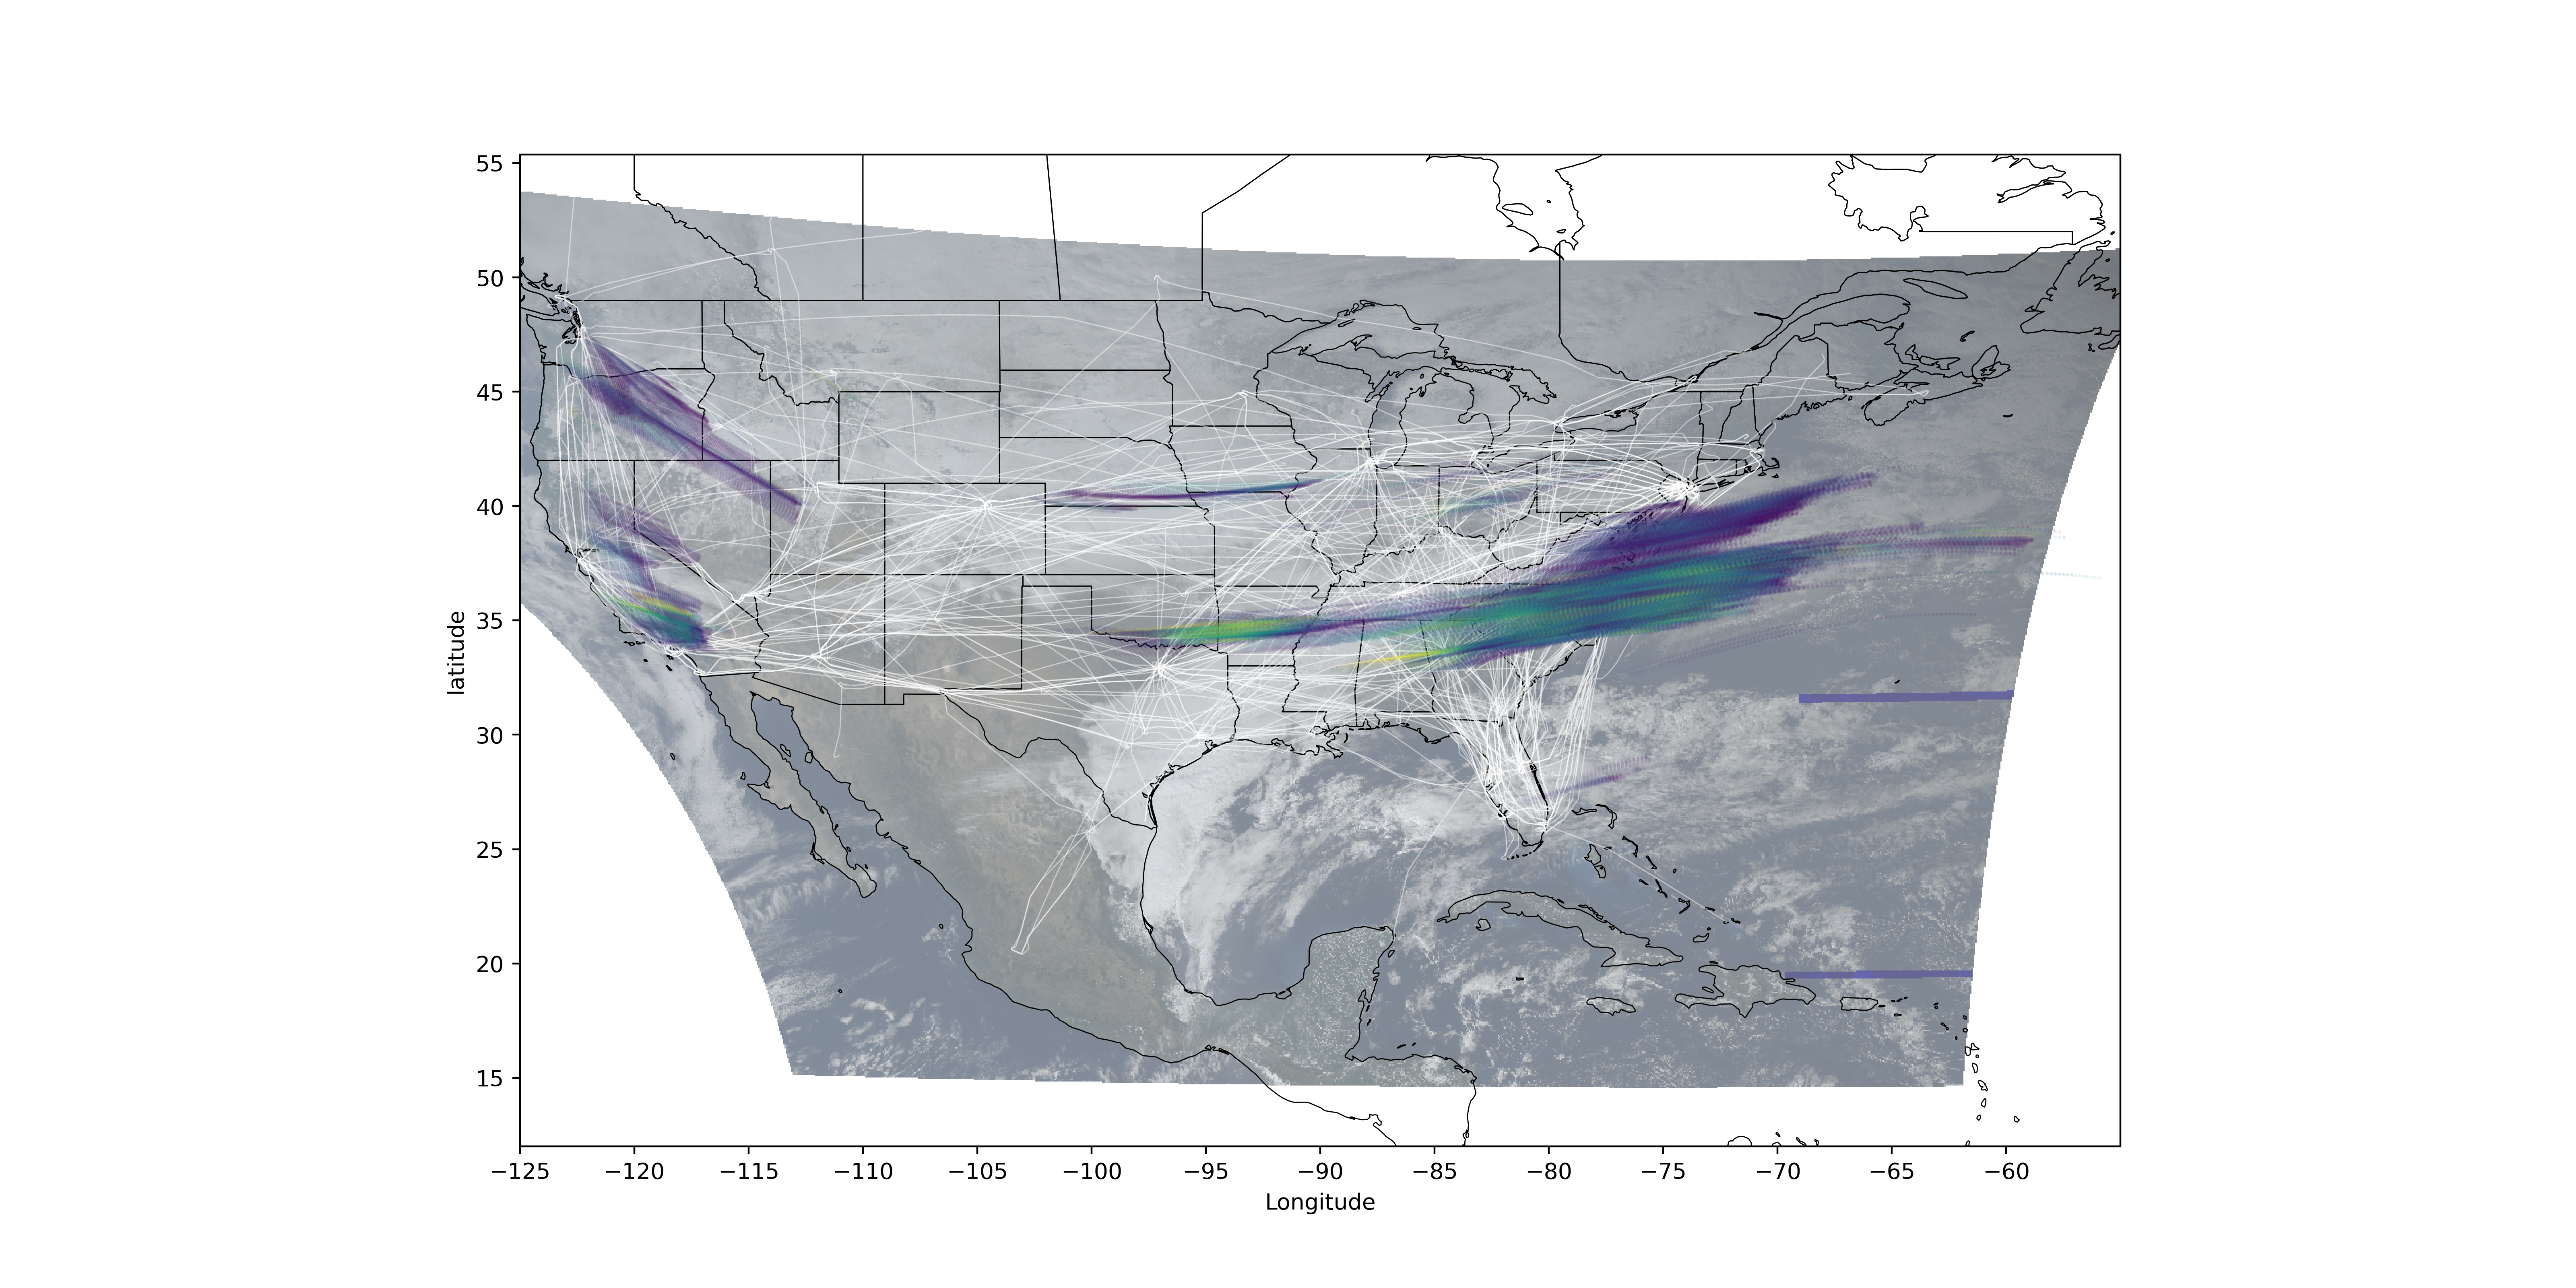
\includegraphics[width=0.99\textwidth]{figures/contrail_map.png}
    \caption{Map of contrails over US produced using CoCiP model provided in pycontrails library \cite{pycontrails}}
    \label{fig:contrail_map}
\end{figure}

\begin{thebibliography}{9}


    \bibitem{co2_modelling}
    R. H. Socolow and S. H. Lam
    \emph{Good enough tools for global warming policy making}
    Department of Mechanical and Aerospace Engineering, Princeton University,
    Princeton, NJ 08544, USA

    \bibitem{rf_greenhouse}
    G. Myhre et al.
    \emph{New estimates of radiative forcing due to well mixed greenhouse gases}
    Geophysical Research Letters, Vol. 25, No. 14, 1998

    \bibitem{contrail_radiative_forcing}
    D. S. Lee et al.
    \emph{The contribution of global aviation to anthropogenic climate forcing for 2000 to 2018}
    Atmospheric Environment, 2020

    \bibitem{pycontrails}
    Marc Shapiro et al.
    \emph{pycontrails: Python library for modelling aviation climate impacts}
    Version v0.54.3 Updated 21 November 2024

\end{thebibliography}

\end{document}